% Chapter Template

\chapter{Project Set-up} % Main chapter title

\label{Chapter 4} % Change X to a consecutive number; for referencing this chapter elsewhere, use \ref{ChapterX}

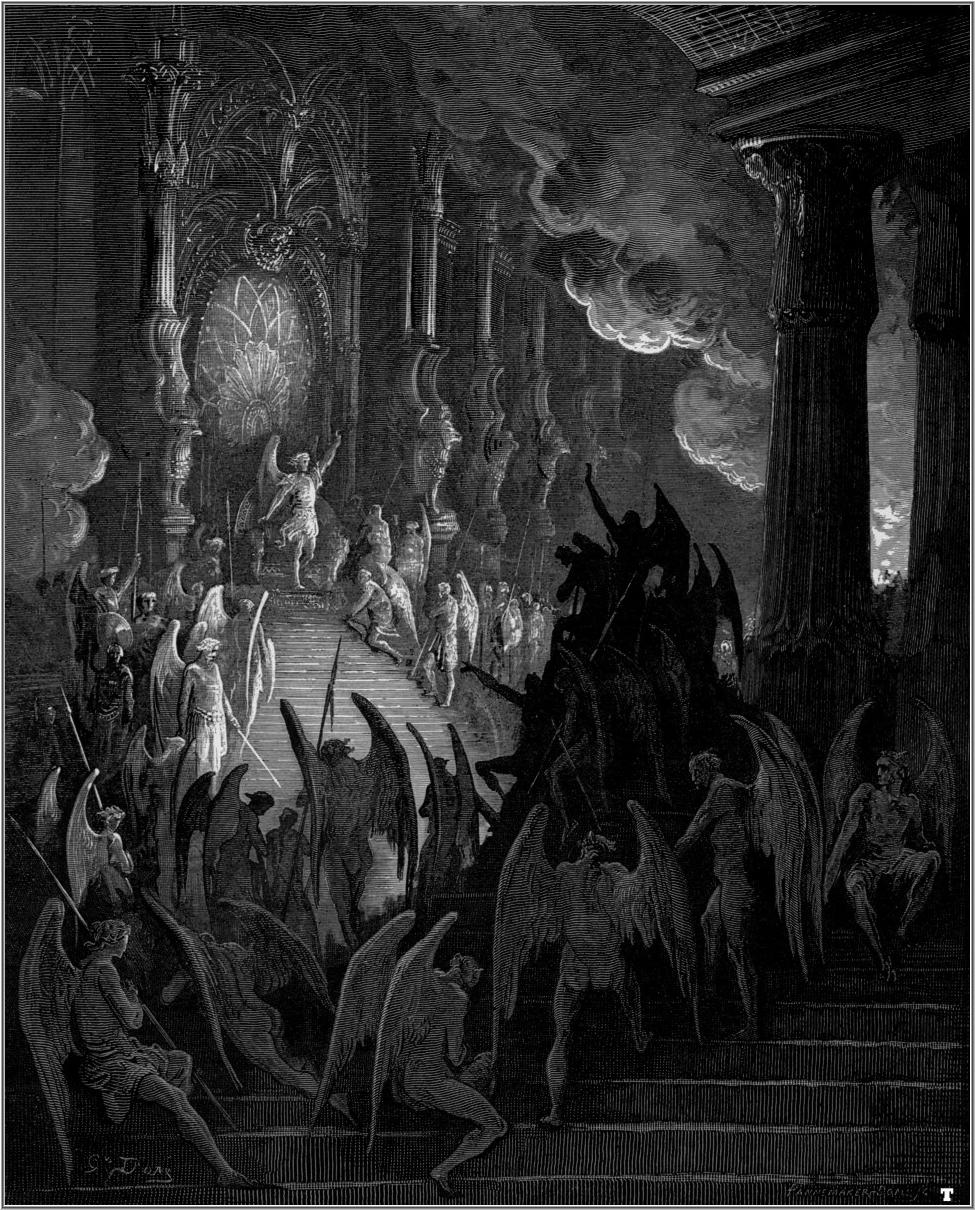
\includegraphics[width=\linewidth,trim={0 12cm 0 7cm},clip]{Paradise_Lost_6}

\section{Overview}

This chapter describes the issues encountered prior to beginning development on answering the research questions posed in section \ref{Ch1 Sec2}. This section start by discussing why there were dependency issues experienced when starting the project. It then goes on to specifically identify the issues and the steps taken to correct these them. Then, in section \ref{Ch4 Sec2}, the issues that were experienced with fdisk are highlighted and the solution discussed. This chapter will end with the final thoughts about the issues encountered and the solutions given. 

%----------------------------------------------------------------------------------------
%	SECTION 1
%----------------------------------------------------------------------------------------

\section{Dependency Issues}

\label{Ch4 Sec1}

The MEGA65 project is an open source project, this works to the benefit, but also to the detriment of the project. Because there are many developers on the project, it is not well documented and the source code is prone to dependency issues that are only problems for newer developers. In addition to the the large developer base, the iterative development cycle and trial and error bug fixing has also caused dependency issues to be present in the source code.

%-----------------------------------
%	SUBSECTION 1
%-----------------------------------
\subsection{Missing Sub-Modules}

\label{Ch4 Sec1 Sub1}

During synthesis errors would often occur due to missing commands that were used in the makefile, but were not natively supported by Ubuntu Linux. The missing commands were the cc65 command, the ca65 command, the ld65 command, cbmconvert command and the ophis command. The cc65 command was used as the C compiler for the 6502 CPU. The ca65 was used in conjunction with the cc65 compiler as the assembler for the 6502 CPU. The ld65 was used as the linker to create an executable file from the object files. In addition to the missing compilation commands the cross-assembler, ophis, and the Commodore binary converter, cbmconvert, commands were not present in the project. These commands were developed separately from the MEGA65 and accessible through their own github repositories. This separation from the MEGA65 project caused each developer to reference the required commands differently, making the use of one universal makefile impossible. In order to correct this, as seen in figure \ref{fig:mega65MakerfileSubmodulesUpdates}, the source code for each required command was initialised as a sub-module of the project. This allowed the making of the project to automatically download, update and build the commands required later during synthesis.\\

\begin{figure}
  \centering
  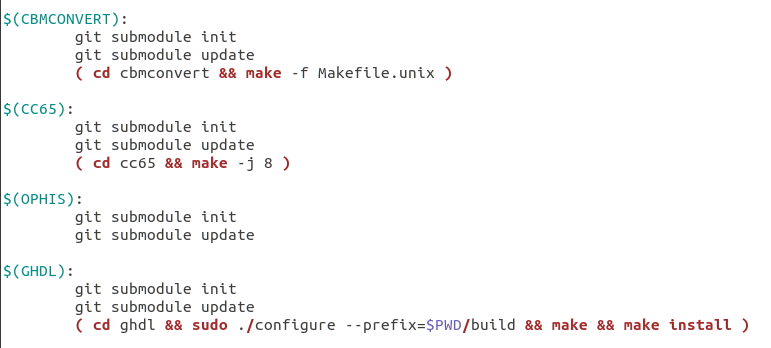
\includegraphics[width=\linewidth]{mega65MakerfileSubmoduleUpdates}
  \caption{The makefile with sub-module initialisation and make additions.}
  \label{fig:mega65MakerfileSubmodulesUpdates}
\end{figure}

Additionally, for these new sub-modules to be used, the pathing in the makefile was changed to correctly reference the required commands. Figure \ref{fig:mega65MakerfilePathing} shows that, thanks to sub-modules being located in the project directory, absolute pathing to the commands can now be done.\\

\begin{figure}
  \centering
  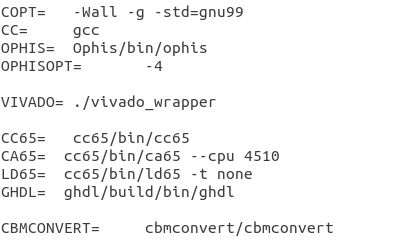
\includegraphics[width=\linewidth]{mega65MakerfilePathing}
  \caption{The updated referencing of the sub-modules}
  \label{fig:mega65MakerfilePathing}
\end{figure}

For the initialising and updating additions to the makefile to be useful, each instance where a sub-module is being used was updated to include a call to the sections seen in \ref{fig:mega65MakerfileSubmodulesUpdates}. One such example of these updates can be seen in figure \ref{fig:mega65AutoBuild}.\\

\begin{figure}
  \centering
  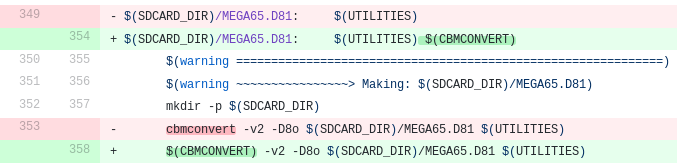
\includegraphics[width=\linewidth]{mega65AutoBuild}
  \caption{The updated function calls that reference the code seen in \ref{fig:mega65MakerfileSubmodulesUpdates}.}
  \label{fig:mega65AutoBuild}
\end{figure}

%----------------------------------------------------------------------------------------
%	SECTION 2
%----------------------------------------------------------------------------------------

\section{Fdisk}

\label{Ch4 Sec2}

In order to partition the MEGA65, the command line tool fdisk was created; this tool was already made a sub-module of the MEGA65 project. Similar to the MEGA65 source code, the fdisk source code had dependency issues in it due to it's open source nature. Specifically, due to the cc65 and cl65 commands being required and the unusuallity of fdisk tool being compiled separately from the MEGA65 project. The pathing for the cc65 and cl65 commands in the mega65-fdisk makefile was incorrect. As seen in figure \ref{fig:fdisk}, previously the cc65 and cl65 commands was just copied into the repository, which was not ideal as the fdisk repository was supposed to be able to be built independently from the rest of the mega65 project. Similar to section \ref{Ch4 Sec1}, the cc65 repository was made a sub-module of the fdisk repository and the fdisk makerfile was changed to automatically initialise it and build it while making fdisk. These changes are shown in figure \ref{fig:fdisk}.\\

\begin{figure}
  \centering
  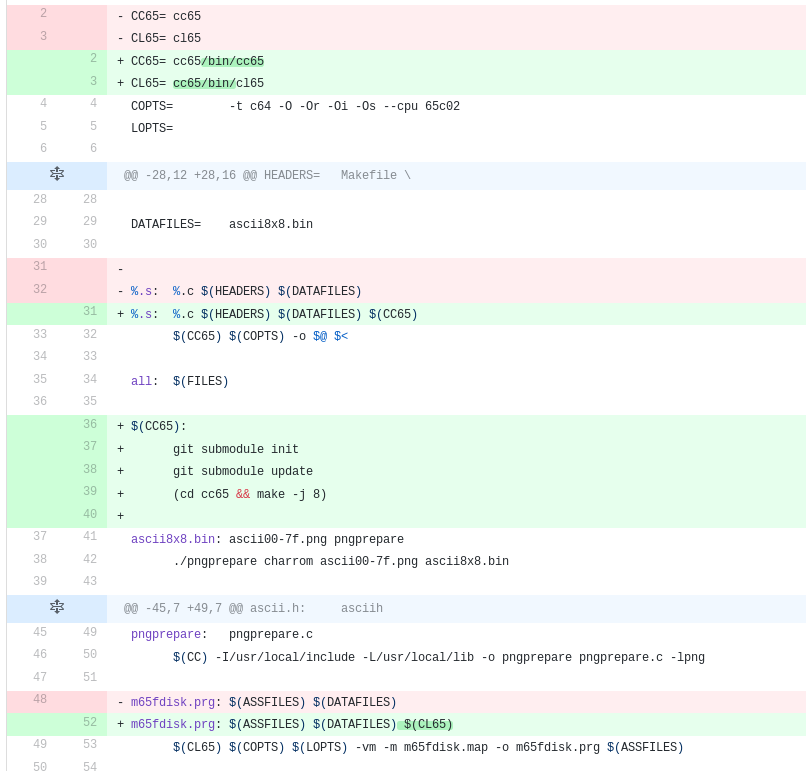
\includegraphics[width=\linewidth]{fdisk}
  \caption{fdisk sub-module dependency changes.}
  \label{fig:fdisk}
\end{figure}

\section{Final Thoughts}

During the start up of the project there were many dependency issues present. This was due to the multiple active branches of the project working at once. Because of this there was no uniform way, in which, the project could be made. In order to correct this issue several third party github repositories were added as sub-modules to the MEGA65 project. In addition, the makefile was changed to update the pathing to the tools used and to automatically download and update these new sub-modules when they were used.
